\section{Introduction}

The number of books published in the U.S. has been on the rise for at least the past decade, only incurring a small setback in 2005\cite{bowker}.
In 2010, Bowker recorded 328,259 new books published in the United States---up from 302,410 during the previous year.
Despite concerns that the paper book is on it's way out, the book publishing industry is still very much a growing one.

% New Books Published per Year Graph
\begin{center}
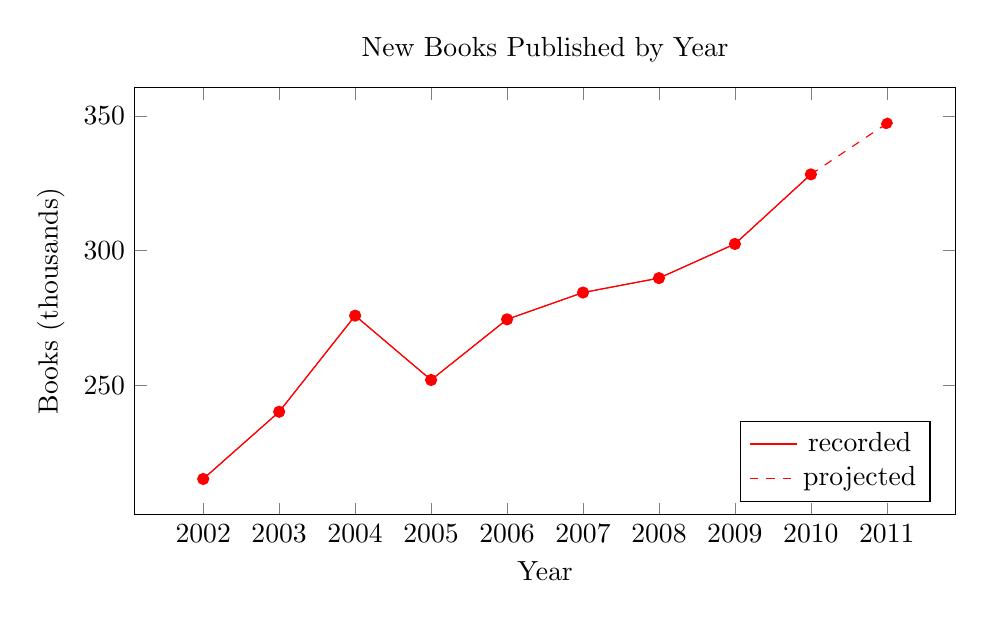
\begin{tikzpicture}
	\begin{axis}[
		title={New Books Published by Year},
		xlabel={Year},
		xticklabel style={/pgf/number format/1000 sep=},
		ylabel={Books (thousands)},
		width=12cm,
		height=7cm,
		legend pos=south east]
		
		\addplot[color=red,mark=,line join=round, solid] coordinates {
			(2002,215.138)
			(2003,240.098)
			(2004,275.793)
			(2005,251.903)
			(2006,274.416)
			(2007,284.370)
			(2008,289.729)
			(2009,302.410)
			(2010,328.259)
		};
		\addplot[color=red,mark=,line join=round, dashed] coordinates {
			(2010,328.259)
			(2011,347.178)
		};
		\addplot[color=red,mark=*,line join=round, solid] coordinates {
			(2002,215.138)
			(2003,240.098)
			(2004,275.793)
			(2005,251.903)
			(2006,274.416)
			(2007,284.370)
			(2008,289.729)
			(2009,302.410)
			(2010,328.259)
		};
		\addplot[color=red,mark=*,line join=round, dashed] coordinates {
			(2011,347.178)
		};
		
		\addlegendentry{recorded}
		\addlegendentry{projected}
	\end{axis}
\end{tikzpicture}
\end{center}

It's a fair assumption that many of these new books also contain an index section between their covers.
An index, of course, is, ``An alphabetical list, placed (usually) at the end of a book, of the names, subjects, etc. occurring in it, with indication of the places in which they occur,'' \cite{oed-index}.
Indexes are popular in non-fiction books, particularly in textbooks.
Readers use indexes to quickly and efficiently locate passages of the book focusing on a specific topic.
Thus, it is important for a book's index to be of high quality, so the reader can locate a particular topic with ease.
A good index can make learning and research easy, while a bad index can result in readers' frustration as they scan over each page in an attempt to find what they are looking for.

\subsection{Cost of Indexing}

The growing number of books published each year and the need for quality indexes in books of all types makes indexing an important sub-industry of the publication process.
Since many books contain indexes, any change in the indexing industry directly affects the publication industry.
If indexing could be made more efficient, the publishing industry could allocate the significant resources that would have gone toward indexing to other, more productive areas.

In {\it Indexing Books}, Nancy Mulvany writes that, ``a typical three-hundred-page book can easily cost close to a thousand dollars to index.
This was in 1994.
Adjusted for inflation using the U.S. Bureau of Labor Statistics' online calculator, \$1,000 dollars in 1994 is equivalent to \$1,578.38 in 2014\cite{inflation-calculator}.
Mulvany goes on to estimate the typical price-per-page at three 1993 U.S. dollars per page in 1994\cite{mulvany}, which is equivalent to \$4.74 in 2014\cite{inflation-calculator}.

The amount of time and money spent on indexing annually can be quantified if a few simplifying assumptions are established.
All rows without citations are conservative guesses for the purpose of estimation:

\begin{center}
\begin{tabular}{|c|l|l|}
\hline
\multicolumn{1}{|c|}{{\bf Symbol}} & \multicolumn{1}{c|}{{\bf Description}} & \multicolumn{1}{c|}{{\bf Statistic}} \\
\hline
$b$ & Number of books published in 2010 \cite{bowker} & 328,259 books \\
\hline
$c$ & Percentage of Books requiring Indexes & 15\% \\
\hline
$d$ & Average dollars per page indexed \cite{mulvany,inflation-calculator} & \$4.74 \\
\hline 
$p$ & Average Number of Pages in Book & 300 pgs \\ 
\hline 
$r$ & Average Number of Pages Indexed per Hour \cite{connolly} & 7 pgs/hr \\
\hline
\end{tabular}
\end{center}

Given these variables, equations are developed to calculate average cost and time impact of manual indexing.

\begin{figure}[H]
$$ \text{cost} = b \times c \times p \times d $$
$$ \text{time} = \frac{b \times c \times p}{r} $$
\\
$$ 69,377,744.70 \text{ USD} = 328259 \times 0.15 \times 300 \times 4.74 $$
$$ 240 \text{ years}= 2,110,236.48 \text{ hours} = \frac{328259 \times 0.15 \times 300}{7}$$
\caption{The Price of Manual Indexing}
\end{figure}

Even with the very conservative assumptions that the average book contains 300 pages and 15\% of books require indexes, the cost of indexing new US books in 2010 was incredibly high.
These numbers reveal the economic impact of indexing, but the individual impact is important too.
If an author wants to index his or her own book, it would take about 42 hours on average. The author could devote an entire work week towards something more productive if there existed an easier way to generate an index.
Clearly, indexing is a significant part of the publishing industry.
natural language processing, a growing specialization of computer science, might be able to reduce these high costs.

\begin{figure}
$$ 42 \text{ hours} = \frac{300}{7} = \frac{p}{r}$$
\end{figure}

\subsection{Natural Language Processing}
% Talk about the rise of natural language processing.

Natural language processing (NLP) is, ``a form of computational linguistics in which natural-language texts are processed by computer (for automatic machine translation, literary text analysis, etc.)''\cite{oed-nlp}.
The sub-discipline of natural language processing (NLP) has existed since the beginning of computers themselves (around 1940), but it has not existed in the modern sense until more recently.
Today, there is a growing focus on machine learning algorithms and processing large amounts of textual data\cite{jurafsky}.
Internet search engines like Google rely on NLP techniques to generate their search results\footnote{As of March 1, 2014, Google has published 219 whitepapers on NLP topics, principally how to use NLP to improve search results.\cite{google-nlp}}, text editing software uses NLP to detect grammatical errors in sentences\cite{norvig}, and mobile applications use NLP to extract summaries from long form text\cite{bit-of-news}.



